\documentclass{beamer}

% Pacotes utilizados
\usepackage[brazil]{babel}
\usepackage[alf]{abntex2cite}
\usepackage{graphicx,hyperref,url}
\usepackage{uegCCETtheme} % pacote customizado para o curso
\usepackage[T1]{fontenc}
\usepackage[utf8]{inputenc}
\usepackage{ragged2e}
\usepackage{subcaption}
\usepackage{tikz, tkz-euclide, tkz-fct}
\usetikzlibrary{babel}
\usetkzobj{all}

% Título da apresentação [título curto]{título longo}
\title[Cálculo Variacional e o Método de Rayleigh-Ritz]{Uma Introdução ao Cálculo Variacional e ao Método de Rayleigh-Ritz com Aplicações em Python}
%\subtitle{Apenas um subtítulo}
% Autores da apresentação [nome curto]{nome longo}
\author[Eduardo José de Oliveira]{
	Eduardo José de Oliveira\\
	Orientador: Prof. Me. Tiago de Lima Bento Pereira
}
% Nome da instituição [nome curto]{nome longo}
\institute[Universidade Estadual de Goiás]{
	UNIVERSIDADE ESTADUAL DE GOIÁS\\
  	Câmpus Anápolis de Ciências Exatas e Tecnológicas Henrique Santillo \\
  	Matemática
}
% Data [data curta]{data longa}
\date[2019]{2019}
% Observação: geralmente o título\autor\data curto é usado
%             em locais como o rodapé enquanto que o título
%             longo é usado em lugares como a capa, por exemplo.

% declara ambientes matemáticos
\newtheorem{definicao}{Definição}
\newtheorem{lema}{Lema}

\begin{document}

	\begin{frame}[plain]
	  \titlepage
	\end{frame}

	\section{Introdução}
	\begin{frame}
		\frametitle{Introdução}
		
		\justify
		Segundo \citeonline{calcvar} e \citeonline{calcvar_campos}, um dos problemas pertinentes ao Cálculo Variacional é o de encontrar uma função diferenciável até a ordem $n$, $y=y(x)$ satisfazendo $y(x_1)=y_1$ e $y(x_2)=y_2$, com $x_1$, $x_2$, $y_1$ e $y_2$ dados, minimizando ou maximizando a integral
		$$
			\int_{x_1}^{x_2} f(x, y, y', y'', \dots, y^{(n)})dx\text{.}
		$$
	\end{frame}
	
	\begin{frame}
		\frametitle{Introdução}
		\justify

		Uma das formas de se encontrar a função $y(x)$ corresponde na determinação da chamada equação de Euler-Lagrange associada ao problema e, então, sua resolução. Além disso, a satisfação das chamadas Condições de Contorno Naturais e Essenciais são necessárias para a correta determinação da função $y(x)$ exata.
		\vspace{10pt}
		\pause
		
		Outra abordagem ao problema consiste na aproximação de $y(x)$ por meio de funções admissíveis.
	\end{frame}
	
	\section{Objetivo}
	\begin{frame}
		\frametitle{Objetivos}
	
		\begin{enumerate}
			\justifying
			\item introduzir, de forma clara e concisa, o Cálculo Variacional por meio do estudo das Equações de Euler-Lagrange para funcionais que dependem de uma única variável, da função e das suas derivadas, até a ordem $n$ desejada;
			
			\item explicar o método de Rayleigh-Ritz, de forma simples e introdutória, desenvolvendo exemplos básicos;
			
			\item apresentar formas de se utilizar a computação para os cálculos do método de Rayleigh-Ritz por meio da linguagem de programação Python.
		\end{enumerate}
	\end{frame}

	\section{Contexto Histórico}
	\makesubtitleframe{Contexto Histórico}

	\begin{frame}
		\frametitle{Máximos e Mínimos}
		\justify
	
		Segundo \citeonline{boyer}, tem-se alguns acontecimentos importantes:
		\begin{itemize}
			\item Pierre de Fermat em 1629.
			\pause
			\begin{itemize}
				\item Comparações entre $f(x)$ e $f(x+E)$ próximo de máximos ou mínimos.
				\pause
				\item Considerar a divisão $\frac{f(x+E)-f(x)}{E}$.
				\pause
				\item Após a divisão, considerar $E=0$.
				\pause
				\item Por último, igualar o resultado a $0$, encontrando as abscissas dos máximos ou mínimos.
			\end{itemize}
			\pause
			\item Cálculo diferencial em 1665 (Isaac Newton) e 1676 (Gottfried Leibniz).
		\end{itemize}
	\end{frame}

	\begin{frame}
		\frametitle{O Problema da Braquistócrona e o Cálculo Variacional}
		\justify
	
		Segundo \citeonline{hist_courant} e \citeonline{hist_still}, o problema da braquistócrona,
		\begin{itemize}
			\item Foi formulado por Johann Bernoulli em 1969 e pode ser apresentado como:
			\begin{block}{Problema da Braquistócrona}
				Sejam $A$ e $B$ dois pontos dados em um plano vertical. O problema da braquistócrona consiste em encontrar a curva que uma partícula M precisa descrever para sair de A e chegar em B no menor tempo possível, somente sob a ação da força da gravidade \cite[p. 3]{calcvar}.
			\end{block}
		\end{itemize}
	\end{frame}

	\begin{frame}
		\frametitle{O Problema da Braquistócrona e o Cálculo Variacional}
		\justify

		Segundo \citeonline{hist_courant} e \citeonline{hist_still},
		\begin{itemize}
			\item A Solução de Jacob Bernoulli (1697) apresenta o aspecto da curva variável.
			\pause
		
			\item Euler e Lagrange.
		\end{itemize}
	\end{frame}
	
	\begin{frame}
		\frametitle{Método de Rayleigh-Ritz}
		\justify
		
		Segundo \citeonline{LEISSA_2005}, 
		\begin{itemize}
			\justifying
			\item o método leva o nome dos pesquisadores Lord Rayleigh e Walter Ritz;
			\pause
			\item estudado, primeiro, por Lord Rayleigh com problemas de energias potencial e cinética de sistemas;
			\pause
			\item generalizado por Walter Ritz;
			\pause
			\item não se sabe exatamente quando o método passou a se chamar "Método de Rayleigh-Ritz".
		\end{itemize}
	\end{frame}
	
	\begin{frame}
		\frametitle{Aplicação do Método de Rayleigh-Ritz}
		\justify

		Uma das aplicações mais usuais nos trabalhos acadêmicos é o seu uso para a determinação das chamadas frequências naturais.
		\vspace{10pt}
		\pause
		
		As frequências naturais "indicam a taxa de oscilação livre da estrutura, depois de cessada à força que provocou o seu movimento. Em palavras similares, representa o quanto à estrutura vibra quando não há força aplicada sobre ela."\text{ }\cite[p. 1]{Vasquez2015}.
	\end{frame}
	
	\begin{frame}
		\frametitle{Aplicação do Método de Rayleigh-Ritz}
		\justify
		
		Essa aplicação pode ser verificada nos trabalhos de 
		\begin{itemize}
			\justifying
			\item \citeonline{RRM_Applications} com as vigas consolas;
			\item \citeonline{mrr_beams} ao estudar a frequência natural em vigas seguindo os modelos de Timoshenko e de Euler;
			\item \citeonline{GROSSI_2001} aplica o método a problemas envolvendo placas.
		\end{itemize}
		\vspace{10pt}
		\pause
		
		\citeonline{deep_ritz} estuda a aplicação do Método junto a Inteligência Aritifical, propondo o método chamado de \textit{Deep Ritz Method} para a resolução de problemas variacionais.
	\end{frame}
	
	\encapsulateBackgroundLessFrames{
		\begin{frame}
			%\frametitle{Aplicação do Método de Rayleigh-Ritz}
			\begin{figure}[h]
				\caption{Solução da equação de Poisson em duas dimensões utilizando o \textit{Deep Ritz Method} e o método das diferenças finitas}
				\centering
				\begin{subfigure}{.4\textwidth}
					\centering
					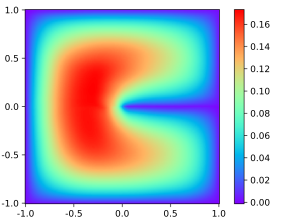
\includegraphics[width=\linewidth]{../figuras/cite/deep_ritz_a.png}
					\caption{Solução pelo \textit{Deep Ritz Method}.}
					\label{fig:deep_ritz_poisson_a}
				\end{subfigure}
				\begin{subfigure}{.4\textwidth}
					\centering
					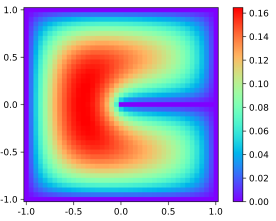
\includegraphics[width=\linewidth]{../figuras/cite/deep_ritz_b.png}
					\caption{Solução pelo método das diferenças finitas.}
					\label{fig:deep_ritz_poisson_b}
				\end{subfigure}
				\label{fig:deep_ritz_poisson}
				\\{\small Fonte: \citeonline[p. 5]{deep_ritz}.}
			\end{figure}
		\end{frame}
	}
	
	\begin{frame}
		\frametitle{Linguagem Python}
		\justify
		
		{\color{red}Colocar tópicos sobre a linguagem de programação Python.}
	\end{frame}

	\section{Cálculo Variacional}
	\makesubtitleframe{Cálculo Variacional}

	%\begin{frame}
	%	\frametitle{Relembrando o problema}
	%	\justify
	%
	%	Deseja-se, no Cálculo Variacional, encontrar uma função diferenciável até segunda ordem $y=y(x)$ satisfazendo $y(x_1)=y_1$ e $y(x_2)=y_2$, com $x_1$, $x_2$, $y_1$ e $y_2$ dados, e $f$ uma função duas vezes diferenciável, minimizando ou maximizando a integral
	%	\begin{equation}
	%		\int_{x_1}^{x_2} f(x,y,y')dx\text{.}
	%		\label{eqn:def_calcvar}
	%	\end{equation}
	%\end{frame}

	%\begin{frame}
	%	\frametitle{Funções Aproximadoras}
	%	\begin{definicao}
	%		\justify
	%		Uma família de funções aproximadoras é definida como
	%		$$Y(x)=y(x)+\varepsilon \eta (x)\text{,}$$
	%		onde a função $\eta (x)$ é uma função diferenciável arbitrária para a qual $\eta (x_1)=\eta (x_2)=0$. O número $\varepsilon$ é o parâmetro da família. Sua derivada pode ser escrita como
	%		$$Y'(x)=y'(x)+\varepsilon \eta '(x)\text{.}$$
	%	\end{definicao}
	%\end{frame}

	\encapsulateBackgroundLessFrames
	{
		\begin{frame}
			\begin{figure}
				\caption{Representação gráfica das funções aproximadoras.}
				\begin{center}
					\resizebox{0.5\textwidth}{0.5\textwidth}{
						\begin{tikzpicture}
	\tkzInit[xmin=-1, xmax=6, ymin=-1, ymax=6]
	% draw axis without ticks
	\tkzDrawX[noticks]
	\tkzDrawY[noticks]
	
	% define extrems on y(x) curve
	\tkzDefPoint[](2.5, 2.0){A}
	\tkzDefPoint[](4.6, 3.76){B}		
	% define helper points
	\tkzDefPoint[](2.5, 0.0){C}
	\tkzDefPoint[](4.6, 0.0){D}
	\tkzDefPoint[](0.0, 2.0){E}
	\tkzDefPoint[](0.0, 3.76){F}
	% helper points to put labels
	\tkzDefPoint[](3.4, 3.2){G}
	\tkzDefPoint[](2.6, 1.7){H}
	\tkzDefPoint[](3.7, 4.2){I}
	\tkzDefPoint[](3.2, 0.4){J}
	
	% draw extrem points on y(x) curve
	\tkzDrawPoint[fill=black, size=7](A)
	\tkzDrawPoint[fill=black, size=7](B)
		
	% y(x)
	\tkzFct[domain=2.5:4.6,samples=1000, line width=2pt]{-exp(-x+3.2)+4}
	% eta(x)
	\tkzFct[domain=2.5:4.6,samples=1000]{-0.18*x*x+1.29*x-2.09}
	% y(x) + 2*eta(x)
	\tkzFct[domain=2.5:4.6,samples=1000,dashed]{-exp(-x+3.2)+4+2*(-0.18*x*x+1.29*x-2.09)}
	% y(x) - 4*eta(x)
	\tkzFct[domain=2.5:4.6,samples=1000,dashed]{-exp(-x+3.2)+4-4*(-0.18*x*x+1.29*x-2.09)}
		
	% draw dotted segments (x_1, y_1), (x_2, y_2)
	\tkzDrawSegment[dotted](A,C)
	\tkzDrawSegment[dotted](B,D)
	\tkzDrawSegment[dotted](A,E)
	\tkzDrawSegment[dotted](B,F)
		
	% x_1, x_2, y_1, y_2 labels
	\tkzLabelPoint[below](C){$x_1$}
	\tkzLabelPoint[below](D){$x_2$}
	\tkzLabelPoint[left](E){$y_1$}
	\tkzLabelPoint[left](F){$y_2$}
	
	\tkzLabelPoint[right](G){$y(x)$}
	\tkzLabelPoint[right](H){$Y_2(x)=y(x)+\varepsilon _2 \eta(x)$}
	\tkzLabelPoint[right](I){$Y_1(x)=y(x)+\varepsilon _1 \eta(x)$}
	\tkzLabelPoint[right](J){$\eta(x)$}
\end{tikzpicture}
					}\\
					{\small Fonte: Elaborada pelo autor, 2019.}
				\end{center}
				\label{fig:func_approx}
			\end{figure}
		\end{frame}
	}
	
	%\begin{frame}
	%	\frametitle{Reescrevendo o Problema}
	%	\justify
	%
	%	Pode-se reescrever a integral \eqref{eqn:def_calcvar} utilizando as funções aproximadoras, dependendo de $\varepsilon$, então
	%	\begin{equation}
	%		\label{eqn:int_funcional_approx}
	%		I(\varepsilon)=\int_{x_1}^{x_2}f(x, Y, Y')dx\text{.}
	%	\end{equation}
	%
	%	Para encontrar a função $y(x)$ que maximiza ou minimiza a integral escrita com as funções aproximadoras \eqref{eqn:int_funcional_approx}, deve-se fazer
	%	$$I'(\varepsilon)=0\text{,}$$
	%	e, considerando que quando $\varepsilon=0$, as integrais \eqref{eqn:def_calcvar} e \eqref{eqn:int_funcional_approx} fornecem os mesmos maximos e mínimos, é necessário que
	%	$$I'(0)=0\text{.}$$
	%\end{frame}

	%\begin{frame}
	%	\justify
	%
	%	Utilizando a Regra de Leibniz, pode-se escrever a derivada de $I(\varepsilon)$ como
	%	$$I'(\varepsilon)=\int_{x_1}^{x_2} \frac{\partial f}{\partial \varepsilon} (x, Y, Y') dx \text{,}$$
	%	\pause
	%	donde, aplicando a regra da cadeia, obtêm-se
	%	$$I'(\varepsilon)=\int_{x_1}^{x_2}\left ( \frac{\partial f}{\partial x}\frac{\partial x}{\partial \varepsilon} + \frac{\partial f}{\partial Y} \frac{\partial Y}{\partial \varepsilon} + \frac{\partial f}{\partial Y'} \frac{\partial Y'}{\partial \varepsilon} \right )dx\text{.}$$
	%	\pause
	%
	%	O primeiro termo do integrando é nulo, pois $x$ independe de $\varepsilon$, então
	%	$$
	%		I'(\varepsilon)=\int_{x_1}^{x_2}\left ( \frac{\partial f}{\partial Y}\frac{\partial Y}{\partial \varepsilon} + \frac{\partial f}{\partial Y'}\frac{\partial Y'}{\partial \varepsilon} \right ) dx \text{.}
	%	$$
	%\end{frame}

	%\begin{frame}
	%	\justify
	%
	%	Derivando a função aproximadora $Y(x)=y(x)+\varepsilon \eta(x)$ em relação a $\varepsilon$, conclui-se que
	%	$$\frac{\partial Y}{\partial \varepsilon}=\eta\text{.}$$
	%	\pause
	%
	%	De modo análogo, ao derivar $Y'(x)=y'(x)+\varepsilon \eta '(x)$ em relação a $\varepsilon$, obtêm-se que
	%	$$\frac{\partial Y'}{\partial \varepsilon}=\eta '\text{.}$$
	%\end{frame}

	%\begin{frame}
	%	\justify
	%
	%	Substituindo $\frac{\partial Y}{\partial \varepsilon}=\eta$ e $\frac{\partial Y'}{\partial \varepsilon}=\eta'$ em $I'(\varepsilon)$,
	%	$$
	%		I'(\varepsilon)=\int_{x_1}^{x_2}\left ( \frac{\partial f}{\partial Y}\frac{\partial Y}{\partial \varepsilon} + \frac{\partial f}{\partial Y'}\frac{\partial Y'}{\partial \varepsilon} \right ) dx
	%	$$
	%	\pause
	%	$$
	%		I'(\varepsilon)=\int_{x_1}^{x_2}\left ( 
	%			\frac{\partial f}{\partial Y} \eta +
	%			\frac{\partial f}{\partial Y'} \eta '
	%		\right )dx \text{.}
	%	$$
	%\end{frame}

	%\begin{frame}
	%	\justify
	%
	%	Calculando $I'(0)$, ou seja, quando $\varepsilon=0$, é possível trocar $Y$ e $Y'$ por $y$ e $y'$, respectivamente, então,
	%	$$
	%		I'(0)=\int_{x_1}^{x_2}\left (
	%			\frac{\partial f}{\partial y} \eta +
	%			\frac{\partial f}{\partial y'} \eta '
	%		\right )dx
	%	$$
	%	\pause
	%	$$
	%		I'(0)=
	%			\int_{x_1}^{x_2} \frac{\partial f}{\partial y}\eta dx
	%			+
	%			\int_{x_1}^{x_2} \frac{\partial f}{\partial y'}\eta' dx \text{.}
	%	$$
	%	\pause
	%
	%	Integrando o segundo membro por partes, tem-se
	%	$$
	%	I'(0)=
	%		\int_{x_1}^{x_2} \frac{\partial f}{\partial y}\eta dx
	%		-
	%		\int_{x_1}^{x_2} \frac{d}{dx} \left ( \frac{\partial f}{\partial y'} \right ) \eta dx
	%	$$
	%\end{frame}
	
	%\begin{frame}
	%	\justify
	%
	%	Organizando $I'(0)$, tem-se
	%	$$
	%		I'(0)=\int_{x_1}^{x_2}\left (
	%			\frac{\partial f}{\partial y} -
	%			\frac{d}{dx}
	%			\left (
	%				\frac{\partial f}{\partial y'}
	%			\right )
	%		\right )\eta dx
	%		\text{.}
	%	$$
	%	\pause
	%	
	%	Devido a condição necessária, $I'(0)=0$, escrevemos
	%	$$
	%		I'(0)=\int_{x_1}^{x_2}\left (
	%			\frac{\partial f}{\partial y} -
	%			\frac{d}{dx}
	%			\left (
	%				\frac{\partial f}{\partial y'}
	%			\right )
	%		\right )\eta dx = 0
	%		\text{.}
	%	$$
	%\end{frame}

	%\begin{frame}
	%	\justify
	%	Para concluirmos a dedução do resultado é necessário o uso do seguinte lema:
	%
	%	\begin{lema}
	%		\justify
	%		Sejam $x_1 < x_2$ fixos e $G(x)$ uma função contínua particular para $x_1 \leqslant x \leqslant x_2$. Se $$\int_{x_1}^{x_2} \eta (x) G(x) dx = 0$$ para cada função diferenciável $\eta (x)$ tal que $\eta (x_1)=\eta (x_2)=0$, concluímos que $G(x)=0$, para todo $x$ de modo que $x_1 \leqslant x \leqslant x_2$.
	%	\end{lema}	
	%
	%\end{frame}

	%\begin{frame}
	%	\frametitle{Equação de Euler-Lagrange}
	%	\justify
	%
	%	Pelo Lema anterior, conlui-se que
	%	$$
	%		\frac{\partial f}{\partial y} - \frac{d}{dx} \left ( \frac{\partial f}{\partial y'} \right )=0 \text{.}
	%	$$
	%	\pause
	%
	%	A equação acima é chamada de \textbf{Equação de Euler-Lagrange}, sendo uma condição necessária para minimizar ou maximizar a integral
	%	$$
	%		\int_{x_1}^{x_2} f(x, y, y')dx \text{.}
	%	$$
	%\end{frame}
	
	\section{Método de Rayleigh-Ritz}
	\makesubtitleframe{Método de Rayleigh-Ritz}
	
	\begin{frame}
		\frametitle{Método de Rayleigh-Ritz}
		
		{\color{red}Explicar o método de Rayleigh-Ritz.}
	\end{frame}
	
	\begin{frame}
		\frametitle{Funções Triangulares}
		
		{\color{red}Explicar o uso das funções triangulares.}
	\end{frame}
	
	\section{Método de Rayleigh-Ritz e a Linguagem Python}
	\makesubtitleframe{Método de Rayleigh-Ritz e a Linguagem Python}
	
	\begin{frame}
		\frametitle{Método de Rayleigh-Ritz e a Linguagem Python}
		
		{\color{red}Explicar sobre o uso da Linguagem Python.}
	\end{frame}

	\section{Referências}
	\begin{frame}[allowframebreaks]
		\frametitle{Referências}
		\bibliography{../references}
	\end{frame}

\end{document}